\section{Vulnerability Seeding}
\label{sec:introduction-of-vulnerabilities-to-code}

\vspace{-0.3cm}

My mission on the SAMATE team consisted in developing the test material for the sixth edition of their \acrlong{sate} with the goal to make it respect the three aforementioned characteristics: relevance, ground-truth and statistical significance.

To achieve our aims, we had to study how to seed vulnerabilities into production software. The following section is a review of the existing methods of bug injection\footnote{~From now on, we will refer to vulnerability addition as bug injection or vulnerability seeding. This area of matter carries indeed various names which are all appropriate}.

\vspace{-0.4cm}

\subsection{Manual Bug Injection}

Existing corpora do not comply with our needs of statistical significance. Indeed, they simply do not provide enough examples to be used as ideal test suites \cite{okun2013report,okun2016sate}. Moreover, most of these corpora are publicly disclosed and therefore have the disadvantage of becoming stale very quickly as we can expect tool vendors to upgrade their analyzers to detect released vulnerabilities. One of the best example is surely the famous ``Heartbleed'' vulnerability: shorlty after the bug was found, two major static analysis tool vendors Coverity and GrammaTech found ways to improve their software so that it could find ``Heartbleed''\dots

But on the other hand, we also specified previously that producing high quality vulnerability corpora is not feasible manually. Surely, manually seeding bugs is the best way to achieve relevance and ground truth, but it takes an insane amount of work to do so. Furthermore, we are still facing the same question: how can we achieve statistical significance?

In fact, creating by hand corpora with a large number of seeded vulnerabilities is a difficult and lenghty process. As a matter of fact, researchers have already been trying before, and it took about six months to produce a very well annotated corpus of only fourteen historic bugs, with triggering inputs \cite{dolan2016lava}.

Injecting bugs manually seems to be unpromising regarding the expected results, because we do not have the time to construct corpora with enough vulnerabilities. However, this is still the best chance we have to seed realistic bugs and produce relevant test cases. We will now discuss other vulnerability addition techniques that have the advantage to be performed in an automated way.

\subsection{Automated Vulnerability Addition}

\subsubsection{Mutation Analysis}

In software testing, fault injection is a popular technique to increase the coverage of test cases by adding faults purposefully in the program's execution paths. There are various ways to implement fault injection, but at a high level picture, two main types of fault injection exist: compile-time injection and run-time injection.

Keep in mind that our goal is not to develop high quality test material in order to verify the correctness of the implementation of a given software system, but to assess the capabilities of static analyzers. As run-time injection consists in triggering faults during execution, is does not modify the source code. As we need to provide effective source code test material, we will just ignore this type of fault injection, and rather focus on compile-time injection.

Compile-time injection entails the modification of the source code in order to seed vulnerabilities in it. Program mutation, also known as mutation testing, is one of these techniques. It involves modifying a program in small ways by changing existing lines of code to make them contain faults \cite{wikipedia2016mutation,wikipedia2016fault}. The idea is to use mutation operators in order to distort the source code, e.g., change all `$+$' operators into `$-$' operators.

Listings \ref{lst:mutation-testing-before} and \ref{lst:mutation-testing-after} show how a small C code fragment could be slightly modified to change the program's behavior. The mutation operator would replace `$\&\&$' with `$||$' and produce a \gls{mutant}, i.e., a mutated buggy version of the original program:

\vspace{0.5cm}

\lstinputlisting
    [
        language=C,
        caption=C code fragment before code mutation \cite{wikipedia2016mutation},
        label=lst:mutation-testing-before
    ]
    {listings/mutation-testing-before.c}

\lstinputlisting
    [
        language=C,
        caption=C code fragment after code mutation \cite{wikipedia2016mutation},
        label=lst:mutation-testing-after
    ]
    {listings/mutation-testing-after.c}

For what we are trying to achieve, mutation testing definitely seems to be a viable option, but the spectrum of vulnerability addition techniques is broader than that. We will discuss now another prominent effort to provide the community with high quality vulnerability corpora: the \gls{iarpa} project \gls{stonesoup} \cite{iarpa2014stonesoup}.

\clearpage

\subsubsection{\gls{iarpa} \gls{stonesoup}}

``The \acrfull{iarpa} project \gls{stonesoup} (\acrlong{stonesoup}) aimed to eliminate the effects of vulnerabilities in software applications by (a) extending the scope and capability of approaches for analysis, confinement, and diversification; (b) addressing a wide range of security vulnerabilities within the same framework; and (c) integrating approaches to leverage the strengths and weaknesses of each. The program aimed to provide comprehensive, automated techniques for vulnerability reduction in software of uncertain provenance'' \cite{iarpa2014stonesoup}.

During phase 3 of the \gls{stonesoup} project, the \gls{iarpa} Test and Evaluation Team developed an automated system to build numerous C and Java test cases with crafted vulnerabilities seeded in a large code base. As they encountered the same issues that emerge when it comes to generate test cases with a great number of realistic vulnerabilities, they embraced the following approach \cite{iarpa2014stonesoup}:

\begin{enumerate}
    \item Selecting and modifying base programs
    \item Developing weakness code with benign and exploiting inputs
    \item Injecting weakness code into the base program
    \item Packaging test cases
\end{enumerate}

The most interesting steps regarding our goals are the second and third one.

\paragraph{What to inject?}

The developers used the \glspl{cwe} defined by MITRE \cite{mitre2016cwe} to design their own weaknesses. For each weakness, T\&E implemented a snippet of code that could be injected into the corresponding program's \gls{ast}, along with triggering inputs as a proof of exploitability.

Into each base program chosen, T\&E implemented (Figure \ref{fig:injected-code}) \cite{iarpa2014stonesoup}:

\begin{enumerate}
    \item An \emph{atomic barrier} to ensure that the vulnerability was run no more than once
    \item A taint source that allowed the user to insert data into the program
    \item Three code complexity features---one each of control flow, dataflow, and data type---to obfuscate the vulnerability
    \item A weakness that acts in either a benign or exploit fashion depending upon user input
\end{enumerate}

\begin{figure}[ht]
    \centering
    \includegraphics[scale=0.43]{figures/injected-code}
    \caption{Code injected into each base program \cite{iarpa2014stonesoup}}
    \label{fig:injected-code}
\end{figure}

\paragraph{How to inject?}

All of this is packed into a code snippet that is converted into an \gls{ast}. Therefore, the bug injection framework would just take multiple files as input, generate their \glspl{ast}, and inject the nodes of the code snippet \gls{ast} into the original source code \gls{ast}. Finally, the modified \glspl{ast} would be unparsed and the new source code would be generated. Figure \ref{fig:injection-process} illustrates the bug injection process.

\begin{figure}[ht]
    \centering
    \includegraphics[scale=0.43]{figures/injection-process}
    \caption{Injection Framework Flow Chart \cite{iarpa2014stonesoup}}
    \label{fig:injection-process}
\end{figure}

\clearpage

\paragraph{Where to inject?}

The last question remaining is where to inject the weaknesses into the \gls{ast}? In order to identify the injection points, T\&E fixed 10 chosen inputs and examined for those 10 inputs which statements in the code would be executed every time.

By proceeding like this, the weaknesses were ensured to be triggerable, whatever the input would be. Figure \ref{fig:injection-points} illustrates the injection points identification process.

\vspace{1.5cm}

\begin{figure}[ht]
    \centering
    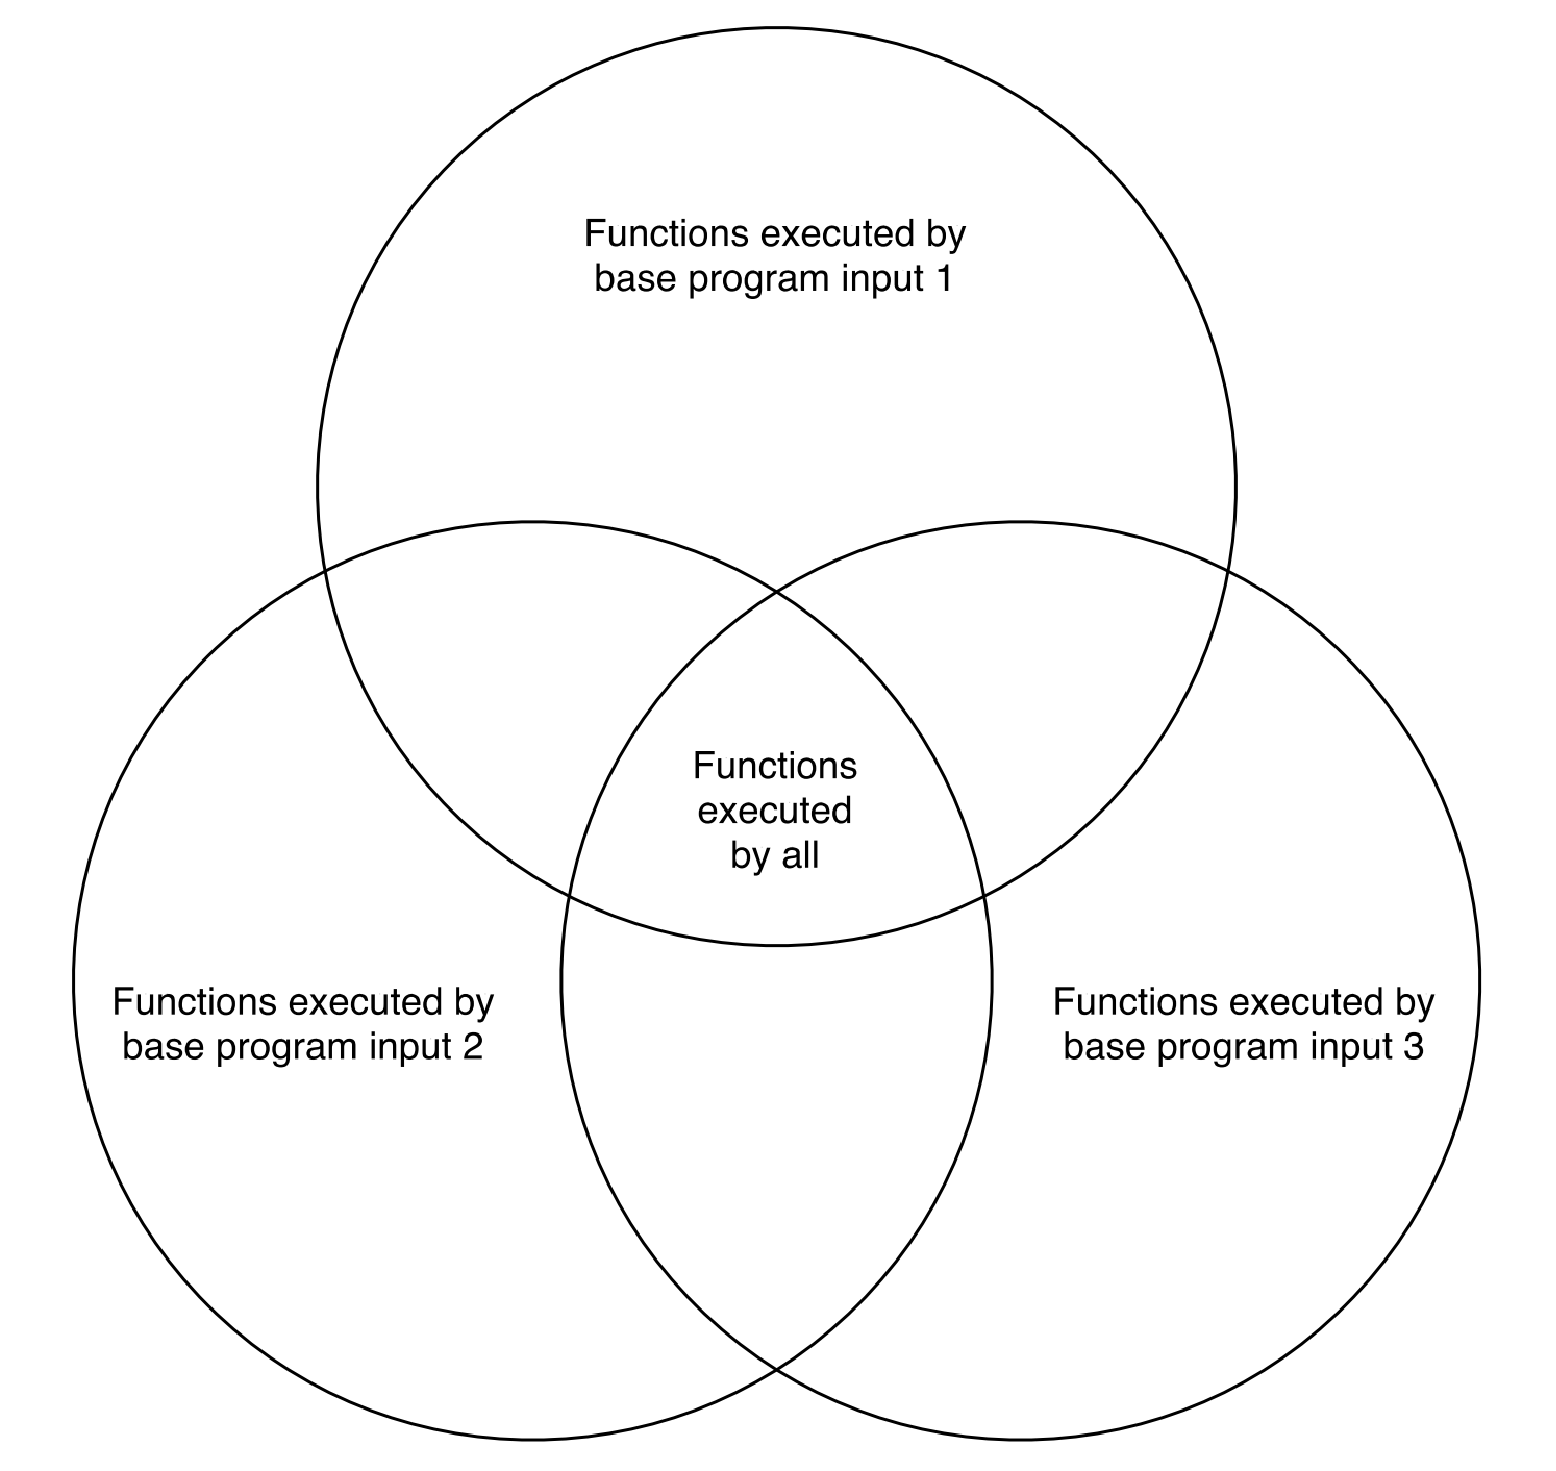
\includegraphics[scale=0.45]{figures/injection-points}
    \caption{Identifying Possible Injection Points \cite{iarpa2014stonesoup}}
    \label{fig:injection-points}
\end{figure}

\vspace{1.5cm}

In closing, \gls{stonesoup} presents a fault injection technique which could be seen as a refined form of code mutation, also known as \emph{Code Insertion Fault Injection}. Code insertion fault injection methods focus on adding code rather than modifying existing one. In a sense, \gls{stonesoup} fault injection method is unique: it adds code snippets, or in other words, cysts, into the source code. These cysts are completely independent from the original program structure.

Lastly, we will present \gls{lava}, yet another \acrlong{lava} method.

\clearpage

\subsubsection{\acrfull{lava}}
\label{sec:lava}

\begin{figure}[ht]
    \centering
    \includegraphics[scale=0.4]{figures/lava-logo}
    \caption{LAVA Logo \cite{dolan2016million}}
    \label{fig:lava-logo}
\end{figure}

\vspace{0.5cm}

Tim Leek from the MIT Lincoln Laboratory came up with  the idea for \gls{lava}. At a high level, \gls{lava} first tries to characterize the program's behavior on concrete input, and then, given an execution trace on some specific input, it adds a large number of bugs.

The governing principle of \gls{lava} resides in its use of \gls{dua} data, and the computation of two very objective metrics: \gls{tcn} and Liveness. To understand the use of \glspl{dua}, one must first understand the bug requirements specified by the \gls{lava} team.

\paragraph{Bugs Properties}We have seen previously that we want our vulnerability corpora to comply with three characteristics: ground truth, relevance and statistical significance. In order to respect these properties, \gls{lava} defines the following requirements for bugs in a vulnerability corpus \cite{dolan2016lava}. Bugs must:

\begin{itemize}
    \item[\textcolor{custom-green}{\ding{51}}] Be cheap and plentiful
    \item[\textcolor{custom-green}{\ding{51}}] Span the execution lifetime of a program
    \item[\textcolor{custom-green}{\ding{51}}] Be embedded in representative control and data flow
    \item[\textcolor{custom-green}{\ding{51}}] Come with an input that serves as an existence proof
    \item[\textcolor{custom-green}{\ding{51}}] Manifest for a very small fraction of possible inputs
\end{itemize}

The first requirement is essential to achieve statistical significance. If we can only add a few bugs per program, then it is not worth to do it automatically \cite{dolan2016lava}.

The second and third requirements are directly related to the relevance property. Bugs should be realistic; whether what that means precisely is a contentious issue. In a nutshell, those two requirements are ``intended to capture the idea that program analyses will need to do essentially the same reasoning about program behavior to find them as they would for any other bugs'' \cite{dolan2016million}.

The fourth is a direct precondition for generated bugs to be considered as real problems. Being able to provide a triggering input that can lead to the exploitability of a weakness is an absolute proof that it is a serious vulnerability \cite{dolan2016lava, dolan2016million}.

Finally, we want to create bugs that are triggered by a limited amount of inputs. Consider a bug that manifests himself for a large fraction of inputs. Then it would be trivially discoverable by simply running the program \cite{dolan2016lava,dolan2016million,dolan2016mechanics}.

\paragraph{\acrfull{dua} Data}

To comply with those requirements, \glspl{dua} form the raw material from which \gls{lava} constructs its bugs. \gls{dua} stands for \acrlong{dua} data:

\begin{labeling}{Uncomplicated}
    \item [\emph{Dead}] The data is actually not used much in the program, which allows to set arbitrary values without mangling the program's behavior.
    \item [\emph{Uncomplicated}] The data is not altered much so we can actually control its value easily.
    \item [\emph{Available}] The data is available in program variables.
\end{labeling}

``We'll call data that satisfies these three properties a \gls{dua}. \glspl{dua} try to capture the notion of attacker-controlled data: a \gls{dua} is something that can be set to an arbitrary value without changing the program's control flow, is available somewhere along the program path we're interested in, and whose value is predictable'' \cite{dolan2016mechanics}.

But the question remains: how can we actually find those \glspl{dua} and make use of it? Finding available data along the program path is not a big deal. For that matter, \gls{lava} performs a dynamic taint analysis on the program, which consists in labeling every byte of every variable and propagating those labels as data is copied around the program. It is thence possible to query any variable and find out if it is derived from some portion of the input data, and if so, from which bytes \cite{dolan2016mechanics}.

Now that we know how to find available data, we still need to identify the dead and uncomplicated ones among them. Well, that is where the \acrfull{tcn} and liveness enter the picture. One handy detail is that those metrics can be computed during the dynamic taint analysis as it goes.

\gls{tcn} is a simple metric tracking the depth of the tree of computation for a value. Every time a variable is modified through some operation, its \gls{tcn} increases. Thus, the smaller the \gls{tcn}, the closer computationally a variable is to the input. In other words, ``\gls{tcn} measures how much computation has been done on a variable at a given point in the program'' \cite{dolan2016mechanics}. This metric is useful to resolve how uncomplicated a variable is.

On the other hand, liveness tracks how many branches use each input byte so we can identify which bytes of the input are actually involved in the execution path decision process. Thus, a \gls{dua} that presents a very low liveness can be accounted as dead data, because it has little influence upon the program's control flow. Figures \ref{fig:taint-compute-number} and \ref{fig:liveness} present the computation process for both metrics.

\begin{figure}[!ht]
    \centering
    \begin{minipage}[t]{7.5cm}
        \centering
        \includegraphics[scale=0.22]{figures/taint-compute-number}
        \caption{\gls{tcn} Computation \cite{dolan2016lava}}
        \label{fig:taint-compute-number}
    \end{minipage}
    \begin{minipage}[t]{8.7cm}
        \centering
        \includegraphics[scale=0.22]{figures/liveness}
        \caption{Liveness Computation \cite{dolan2016lava}}
        \label{fig:liveness}
    \end{minipage}
\end{figure}

By performing a dynamic taint analysis on the program, and computing for every labeled data the \gls{tcn} and liveness metrics, \gls{lava} has the capability to find the \glspl{dua} in the source code. At that point, \gls{lava} has potential attacker-controlled data . Therefore, the next step is to find the locations in the source code where the \glspl{dua} can be used to trigger a vulnerability, i.e., the \glspl{atp}.

The \glspl{atp} selection depends on the type of vulnerabilities we want to inject. It only requires some location in the code where we can actually use the \gls{dua} to trigger a buggy effect. For that reason, it is obvious that the \gls{atp} should be ``temporally after'' an appareance of a DUA in the trace \cite{dolan2016lava}. The current state of implementation of \gls{lava} focuses on overflow issues and therefore examine the code for locations where pointers are passed into functions. The \glspl{dua} are used to modify the pointer, therefore causing out of bounds read or write operations \cite{dolan2016mechanics}.

Notice that we still want bugs that manifest for a small fraction of the possible inputs. Just like \gls{stonesoup} and its injection of atomic barriers to ensure bugs trigger for single inputs, \gls{lava} has its own way to reduce the scope of inputs that can trigger the generated bugs. For each bug, \gls{lava} makes sure that the \gls{dua} matches a specific value in order to trigger the bug.

In a nutshell, a bug generated by \gls{lava} is a combination pair of a \gls{dua} and an \gls{atp} (Figure \ref{fig:lava-bug}). ``Any $(DUA,ATP)$ pair where the DUA occurs before the attack point is a potential bug we can inject'' \cite{dolan2016mechanics}.

\vspace{0.5cm}

\begin{figure}[ht]
    \centering
    \includegraphics[scale=0.35]{figures/lava-bug}
    \caption{LAVA Bug ``Formula'' \cite{dolan2016mechanics}}
    \label{fig:lava-bug}
\end{figure}

\vspace{0.5cm}

We will see how I got to work much further on the \gls{lava} software. Therefore, we will give more information on the technical aspects of the \gls{lava} implementation in Section \ref{cpt:design-of-the-solution}.